\section{Introduzione}
\subsection{Che cos'è un sistema operativo?}
Un sistema operativo è una componente software che si pone tra l'hardware e le applicazioni e:
\begin{itemize}
    \item facilita lo sviluppo e la portabilità degli applicativi: il SO astrae alcuni concetti propri dell'hardware fornendo delle interfacce per l'utilizzo tramite le \emph{chiamate a sistema} (system call o primitive), queste sono dette API (Application Programming Interface). Ad esempio l'astrazione del \emph{file system} ci svincola dall'interfacciarci direttamente con lo storage di massa fornendoci una visione più ad alto livello quale quella dei file e delle directory.
    
    \item gestisce le risorse del sistema di elaborazione: si occupa di associare le risorse a chi le chiede, gestire la mutua esclusione se ve ne è necessità, sincronizzare gli accessi
    
    \item fornisce meccanismi di protezione, garantisce la sicurezza del sistema e la tolleranza ai guasti: memoria virtuale, privilegi dei processi, utenti e gruppi, permessi sui file e sui dispositivi
\end{itemize}

Le API di fatto generano una \emph{macchina astratta} standard che permette a chi sviluppa le applicazioni di non preoccuparsi di cosa c'è sotto in quanto le interfacce sono standard. A cambiare sarà l'implementazione di queste interfacce che tuttavia è competenza del programmatore di sistema.

\subsection{Cenni storici}

\subsubsection{Primi calcolatori}
I primi calcolatori erano pensati per i centri di ricerca, chi li usava erano fisici e matematici che scrivevano il loro software di calcolo su delle schede perforate che venivano consegnate agli addetti alla macchina che si occupavano di caricare le schede in memoria e lanciare il programma.
I risultati poi venivano forniti attraverso altre schede perforate o tramite altri supporti.
Un programma per volta poteva essere eseguito e bisognava aspettare la fase di caricamento, di esecuzione e di "stampa" prima di poterne caricare un altro.

\subsubsection{Sistemi batch monoprogrammati}
Per migliorare l'efficienza dei calcolatori esistenti si inizia ad introdurre una \emph{memoria di massa} (nastri magnetici), questo per poter leggere le schede e salvarle in memoria di massa.
Il programma viene quindi caricato prima su memoria di massa e da lì poi in memoria ed eseguito, successivamente anche il risultato viene salvato su memoria di massa, pronto per essere estratto e stampato a schermo o con altri mezzi.
Si inizia ad avere un po' di parallelismo in quanto finché il calcolatore sta eseguendo un job posso caricarne un altro in memoria di massa!
Assieme a questo la memoria inizia ad essere più grande quindi oltre al programma applicativo si carica un primordiale sistema operativo che implementa un \emph{Job Control Language} (JCL), una specie di linguaggio di shell che permette di scrivere dei comandi da impartire al sistema.
Oltre a produrre le schede del programma si aggiugono alcune schede con comandi JCL per, ad esempio: compilare e poi eseguire passando determinati dati. Questo insieme di schede è detto \emph{batch}.

Oltre al JCL il sistema operativo ha un BIOS (Basic Input Output System) che fornisce delle funzionalità di input ed output più astratte.

In fine un'ultima rivoluzione importante è l'introduzione del DMA: ora possiamo inviare dati in output o prendere dati in input in memoria senza passare per la CPU, la macchina è enormemente più efficiente.

Siamo davanti ancora ad un sistema monoprogrammato ma siamo già molto più efficienti.

Alcuni problemi di questo sistema riguardano i bound del programma:
\begin{itemize}
    \item CPU bound: è un programma che usa molta CPU e poco I/O
    \item I/O bound: è un programma che usa molto l'I/O e poco la CPU
\end{itemize}
se abbiamo molti programmi I/O bound allora gran parte del tempo del calcolatore sarà sprecato ad aspettare che queste operazioni finiscano.

\subsubsection{Sistemi di Spooling}
Sono sistemi che implementano lo spool (simultaneous peripheral operation on-line) cioè sistemi che permettono più flussi di dati contemporaneamente:
\begin{itemize}
    \item posso leggere le schede e metterle in memoria
    \item spostare i dati dalla memoria al disco
    \item spostare i dati dal disco alla memoria
    \item spostare i dati dalla memoria ad una stampante
\end{itemize}
il tutto contemporaneamente e spesso con l'ausilio del DMA. Abbiamo ancora un aumento dell'efficienza ma continuano ad esserci problemi di spreco di tempo.

\subsubsection{Sistemi multiprogrammati}
Introduciamo la gestione di più programmi, carichiamo in memoria più di un programma, facciamo partire il primo, quando il primo richiede l'utilizzo dell' I/O lo stoppiamo e mettiamo in esecuzione il secondo, e così via. La CPU è usata in maniera molto più efficiente in quanto i tempi morti dell'I/O sono ridotti al minimo. Questo comportamento aggiunge complessità al sistema operativo che ora deve poter salvare lo stato di un job, ripristinarlo, gestire le periferiche e gestire lo scheduling dei processi, cioè come scegliere quale processo far andare prima degli altri disponibili.

Con l'esecuzione sequenziale abbiamo:
\begin{figure}[H]
    \centering
    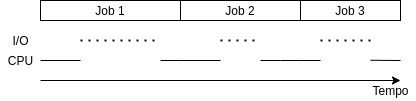
\includegraphics[width=300px]{images/1_Introduzione/esecuzione_sequenziale.png}
\end{figure}

Con l'esecuzione in multi-tasking abbiamo:
\begin{figure}[H]
    \centering
    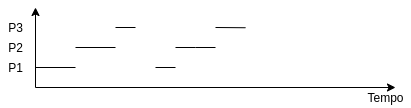
\includegraphics[width=300px]{images/1_Introduzione/esecuzione_multi_tasking.png}
\end{figure}

Si nota a prima vista la maggiore efficienza del secondo metodo!

Questi primi sistemi multiprogrammati non supportano la preemption cioè: se un processo parte la CPU rimane sua finché il processo stesso non si blocca per qualche motivo, il sistema operativo non può interromperlo in nessun modo.
La preemption inizia ad essere presente con l'introduzione delle interruzioni: chiedo all'hardware di fare qualcosa, quando l'hardware ha finito me lo fa sapere tramite un segnale, il sistema operativo lo gestisce e rimette in esecuzione il programma stoppato.
Questo comportamento è molto utile per revocare il tempo macchina a processi \emph{number-crunching} ed ottimizzare meglio lo scheduling rispetto ad altre metriche.

Un problema della multiprogrammazione è l'aggiunta di overhead, il cambio di processo prevede il salvataggio dello stato del primo ed il ripristino dello stato del secondo, a volta bisogna cambiare anche il contenuto della memoria per ripristinare la memoria utilizzata dal processo, questo può essere dispendioso in termini di tempo.

\subsubsection{Sistemi time-sharing}
Una delle modalità di revoca (preemption) prevede la suddivisione del tempo in slot, \emph{quanti} di tempo, predefiniti.
La CPU è assegnata ad un processo per un quanto di tempo, allo scadere del quanto revoco e cambio processo.
Diminuisce l'overhead in quanto non deve fare un vero e proprio scheduling poiché basta utilizzare una politica FIFO, un round robin.
Questo è possibile utilizzando un timer configurato a dovere per lanciare una interruzione ad intervalli costanti.

Ovviamente se il processo finisce nel mezzo del quanto o richiede l'utilizzo dell'I/O nel mezzo del suo tempo di CPU esso viene stoppato, si passa al prossimo e si resetta il contatore del timer.

Un processo quindi si stoppa in queste 3 occasioni.

\subsubsection{Sistemi in tempo reale (RTOS)}
Sono sistemi operativi molto leggeri pensati ed utilizzati per dispositivi che devono rispondere velocemente agli stimoli esterni, si parla quindi di applicazioni all'interno di microcontrollori e sistemi embedded.
Arriva uno stimolo dall'esterno tramite un sensore, velocemente il sistema produce una risposta e la fornisce in uscita tramite degli attuatori.

Questi sistemi operativi devono garantire risposte agli stimoli entro un determinato tempo, detto \emph{deadline}. Per queste caratteristiche non si può usare un time sharing perché potrebbe non rispettare tutte le deadline, bisogna pertanto utilizzare algoritmi di scheduling più efficienti e basati sulla priorità dei job.

Classifichiamo questi sistemi operativi in:
\begin{itemize}
    \item Hard: dato un insieme di task, ognuno con le sue deadline ed il suo periodo (task periodici), devo garantire che tutti i task eseguano senza violare la deadline. Es: dei controllori per la guida assistita.

    \item Soft: posso permettermi di violare qualche deadline con un peggioramento della qualità del servizio. Es: dei controllori per dispositivi multimediali, posso permettermi di avere il video al televisore un po' in ritardo, non succede niente, al massimo pecca un po' di qualità video.
\end{itemize}

\subsection{Componenti del sistema operativo}
Un sistema operativo moderno si compone almeno delle seguenti componenti:
\begin{itemize}
    \item gestore dei processi
    \item gestore della memoria principale
    \item gestore dei dispositivi periferici
    \item gestore dei file
    \item gestore delle comunicazioni sulla rete
    \item interprete del linguaggio di controllo
\end{itemize}

Queste componenti possono essere arrangiate in maniera diversa dando vita a diverse architetture kernel.

\subsubsection{Struttura monolitica}
Tutto il sistema operativo è un singolo software, viene allocato tutto assieme nella stessa zona di memoria.
E' difficilmente scalabile, è difficilissimo sostituire una singola componente senza rompere tutto il resto.
Al crescere delle dimensioni e delle funzionalità diventa sempre più importante la modularità

\subsubsection{Struttura modulare - UNIX}
Unix è un primo esempio di sistema operativo modulare, si divide in 4 macro blocchi: utente, utilities, kernel ed hardware.
\begin{figure}[H]
    \centering
    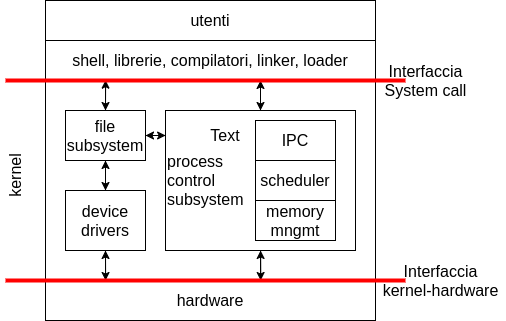
\includegraphics[width=300px]{images/1_Introduzione/monolith.png}
\end{figure}

Il kernel UNIX inoltre è diviso in altri singoli blocchi che si occupano ognuno di una cosa specifica, tra questi blocchi nominiamo:
\begin{itemize}
    \item Process control subsystem: si occupa della gestione dei processi, della loro creazione, del loro scheduling, della gestione della loro memoria e della loro comunicazione
    \item File subsystem: costruisce l'astrazione del file system e rende accessibili i file tramite le primitive
    \item Device driver: sono i driver che si occupano di parlare con le periferiche, di gestirne l'accesso esclusivo, la coerenza, ecc.
\end{itemize}

La comunicazione tra l'utente ed il sistema avviene solamente tramite le system call messe a diposizione dal sistema operativo stesso.

Questa struttura a livelli gerarchici è generalizzabile a N livelli: ogni livello dialoga con il precedente usando le sue API e dialoga con quello successivo mettendo a disposizione altre API.

NB: chi fornisce una interfaccia è detto \emph{provider}, chi usa una interfaccia è detto \emph{user} dell'interfaccia.

\subsubsection{Struttura a microkernel}
L'idea è di inserire nel kernel solo i meccanismi necessari al funzionamento generale del sistema operativo, il resto dei meccanismi vengono implementati separatemente. In questa struttura non tutte le componenti girano a livello sistema.
\begin{figure}[H]
    \centering
    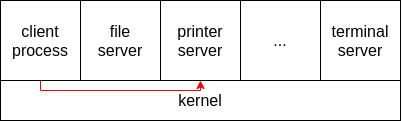
\includegraphics[width=300px]{images/1_Introduzione/microkernel.png}
\end{figure}
Se un processo vuole accedere al file system usa il kernel per contattare il file server.

\subsubsection{Struttura client-server}
Il sistema operativo è distribuito su diverse macchine e la comunicazione avviene tramite qualche protocollo di rete.
\begin{figure}[H]
    \centering
    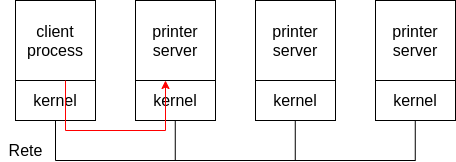
\includegraphics[width=330px]{images/1_Introduzione/network-kernel.png}
\end{figure}

